\section{LTI System Stability Analysis and Modification}
Consider the LTI system described by the following difference equation:

$$y(n)-1.2y(n-1)+0.8y(n-2)=x(n)$$

Question:

\begin{enumerate}
	\item Determine if this system is stable or not
	\item Plot poles and zeros of the system
	\item Compute and plot the impulse response of the system for $0\le n\le 50$
	\item Modify the system by changing the coefficient of $y(n-1)$ and $y(n-2)$ so that the poles are located at $p=0.5\pm 0.5j$. Plot the pole-zero diagram for new system
\end{enumerate}

\subsection*{Program for Question 1-3:}

\importMLCode{code/Q21.m}


\begin{figure*}[ht!]
	\begin{minipage}{.45\textwidth}
		\inc{Q21.pdf}
	\end{minipage}%
	\hfill%
	\begin{minipage}{.45\textwidth}
		\inc{Q22.pdf}
	\end{minipage}
\end{figure*}

\hrule
\subsection*{Program For Question 4}
\vspace*{10pt}

Given system has 2 zeros at $p = 0$ and 2 poles. To change the poles location to $p=0.5\pm 0.5j$, First write it in system function form, change denominator expressions and work backwards: (here $z^2$ implies double zero at $p = 0$)
\begin{align*}
	H'(z) &= \frac{z^2}{(z - p_1)(z - p_2)}\\
	H'(z) &= \frac{z^2}{
		\left[z - \left(0.5 + 0.5i\right)\right]
		\left[z - \left(0.5 - 0.5i\right)\right]
	} \\
	 &= \frac{z^2}{z^2 -1z + 0.5} \\
	 \frac{Y(z)}{X(z)} &= \frac{1}{1 -1z^{-1} + 0.5z^{-2}} \\
	 \Rightarrow X(z) &= Y(z)\left[1 -1z^{-1} + 0.5z^{-2}\right]
\end{align*}

Applying inverse Z-transform gives the required system:
$$x(n) = y(n) - y(n - 1) + 0.5y(n - 2)$$
Hence the implementation: 
\importMLCode{code/Q22.m}
\begin{figure*}[ht!]
	\centering
	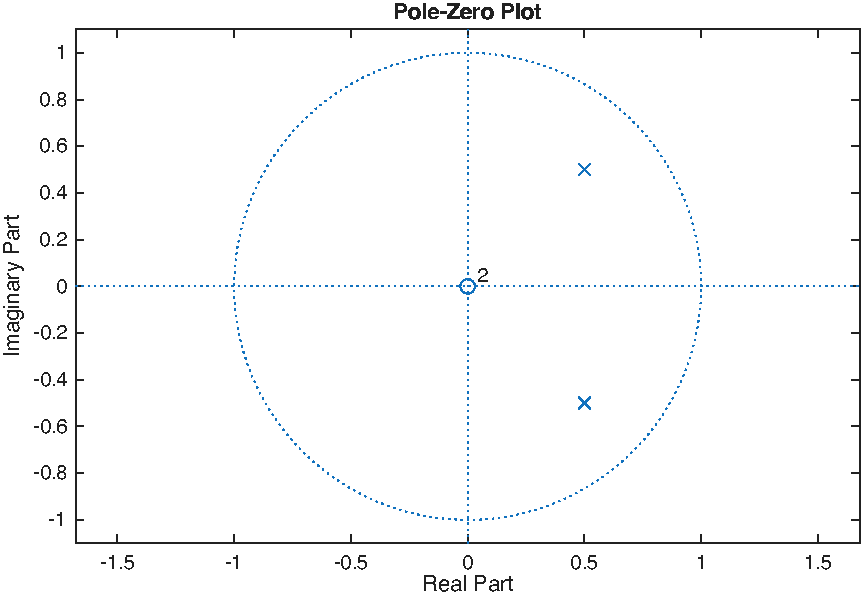
\includegraphics[width=.5\textwidth]{img/Q23.pdf}
	\caption*{new system function}
\end{figure*}